\documentclass[twocolumn]{article}
\usepackage{graphicx}

\title{Varlens: annotating a personal genome on the computer you have}

\begin{document}
\maketitle

\begin{abstract}
Varlens annotates one whole-genome variant file locally, without uploading it, in a median of 31.4 seconds
on a desktop computer and in under four minutes on a Raspberry Pi 5. Each result names the studies behind it.
\end{abstract}

\section{Introduction}

People who receive their genome as a variant file cannot read it, and the services that can read it ask them
to upload it. Varlens reads the file on the user's own computer and shows, for each annotated variant, the
association and the studies that report it (Figure~\ref{fig:report}).

\begin{figure}
  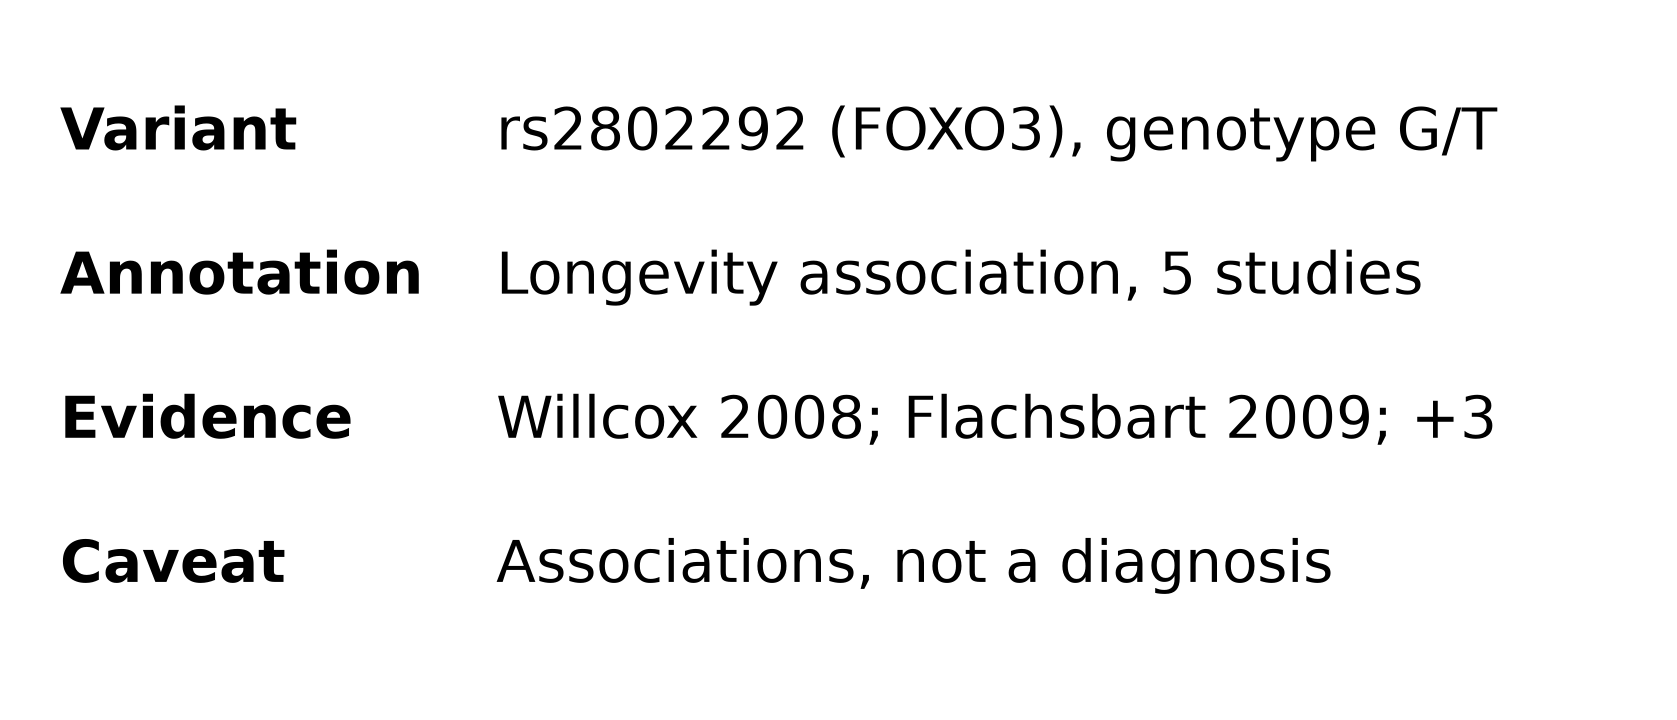
\includegraphics[width=\columnwidth]{figures/report}
  \caption{One row of a Varlens report, as a user sees it: the variant and genotype, the annotation, the
  studies behind it and the caveat shown with every association.}
  \label{fig:report}
\end{figure}

\section{Methods}

Varlens joins the variants of a VCF file with annotation tables by chromosome, position and allele. We timed
five runs of each tool on one whole-genome VCF (4.6 million variants) and report the median. During one run
on the desktop computer (12 threads) we recorded resident memory and the number of busy threads every 2 s.

\section{Results}

\subsection{Speed}

On the desktop computer, Varlens annotated the genome in a median of 31.4~s, against 940~s for the server
annotator and 5,712~s for the previous pipeline (Figure~\ref{fig:runtime}).

\begin{figure*}
  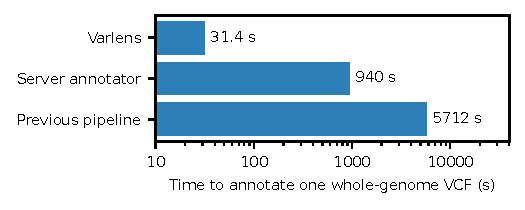
\includegraphics[width=\textwidth]{figures/runtime}
  \caption{Time to annotate one whole-genome VCF with each tool on the desktop computer: the median of five
  runs, on a logarithmic scale.}
  \label{fig:runtime}
\end{figure*}

\subsection{Four computers}

Varlens needs no server. On the four computers we tried, the median time to annotate the genome was 21.3~s on
a workstation with 32 threads, 31.4~s on the desktop computer with 12 threads, 44.0~s on a laptop with 8
threads and 212.6~s on a Raspberry Pi 5 with 4 threads; peak resident memory was 2.2, 2.1, 2.0 and 1.9~GB.

\subsection{Resources}

Resident memory stayed at or below 2.1~GB during the run (Figure~\ref{fig:memory}), and all twelve threads
were busy within 4~s and stayed busy until the last tables were joined (Figure~\ref{fig:threads}).

\begin{figure}
  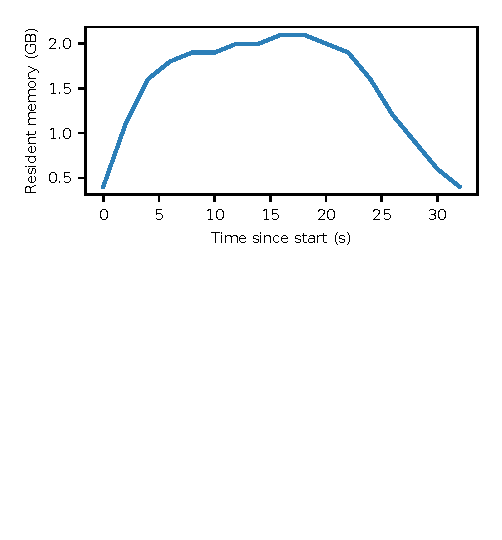
\includegraphics[width=\columnwidth]{figures/memory}
  \caption{Resident memory of Varlens during one annotation run on the desktop computer, sampled every 2 s.}
  \label{fig:memory}
\end{figure}

\begin{figure}
  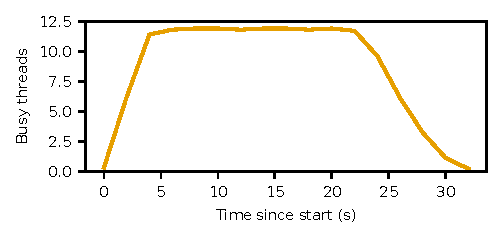
\includegraphics[width=\columnwidth]{figures/threads}
  \caption{Busy threads of Varlens during the same run, sampled every 2 s; the desktop computer has 12.}
  \label{fig:threads}
\end{figure}

\subsection{Agreement}

Table~\ref{tab:agreement} compares the annotations with a manually curated reference.

\begin{table}
  \caption{Agreement with the curated reference set (2,184 variants).}
  \label{tab:agreement}
  \begin{tabular}{lrr}
    \hline
    Tool & Agreement & Disagreement \\
    \hline
    Varlens & 2,171 (99.4\%) & 13 \\
    Server annotator & 2,160 (98.9\%) & 24 \\
    \hline
  \end{tabular}
\end{table}

\section{Discussion}

Varlens makes a personal genome readable on the computer its owner already has. It reports associations, not
diagnoses, and its annotations are only as current as the tables it joins.

\end{document}
